%
% fig-stereowechsel.tex
%
% (c) 2024 Prof Dr Andreas Müller
%
\begin{figure}
\centering
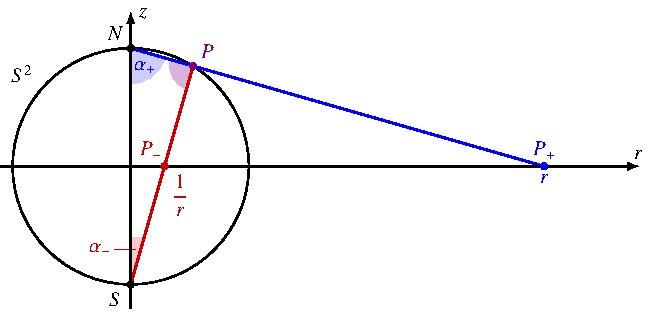
\includegraphics{chapters/020-koordinaten/images/stereowechsel.pdf}
\caption{Die stereographische Projektion $\varphi_+$ vom Nordpol
der Kugel aus bildet den Kugelpunkt $P$ auf den Punkt $P_+$ ab, die 
stereographische Projektion vom Südpol bildet ihn auf $P_-$ ab.
Die Kartenwechselabbildung $\varphi_-\circ\varphi_+^{-1}$ bildet $P_+$
auf $P_-$ ab.
Da $P$ auf dem Thales-Kreis über der Strecke $NS$ liegt, ist der Winkel
bei $P$ ein rechter Winkel und die Winkel $\alpha_+$ und $\alpha_-$
sind komplementär.
Es folgt, dass das Produkt der $r$-Koordinaten der Punkte $1$ ist.
\label{buch:koordinaten:diffmannig:fig:stereowechsel}}
\end{figure}
